\textcolor{black}{\section{Procedimiento}}

\begin{figure}%[H]
	\centering
	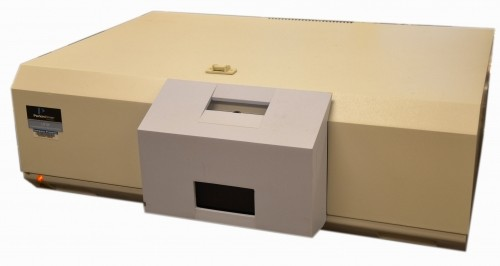
\includegraphics[scale=0.4]{figs/PELS55.jpg}
	\caption{Perkin Elmer LS55 Luminsescence Spectrometer. \cite{PELS55}}
	\label{fig:PerkinELmer}
\end{figure}

\begin{figure}%[H]
	\centering
	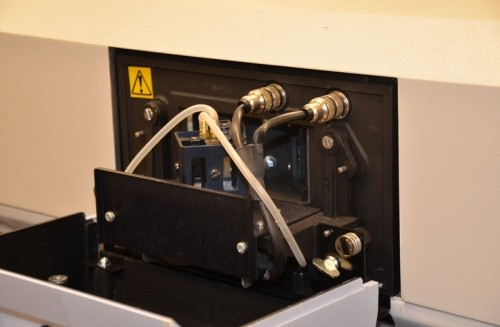
\includegraphics[scale=0.4]{figs/abertura.jpg}
	\caption{Compartimiento para colocar las muestras en un espectrómetro Perkin Elmer LS55 Luminsescence Spectrometer. \cite{PELS55}}
	\label{fig:abertura}
\end{figure}

\begin{figure}%[H]
	\centering
	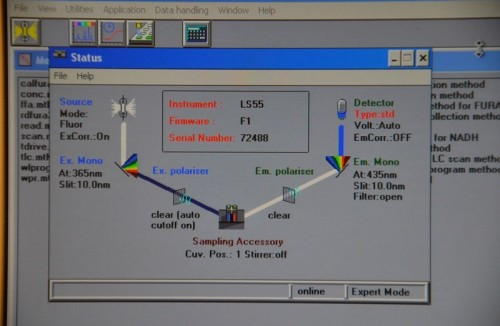
\includegraphics[scale=0.4]{figs/FL_Winlab.jpg}
	\caption{Software FL Winlab; para manejar el espectrómetro Perkin Elmer LS55. \cite{PELS55}}
	\label{fig:FL_Winlab}
\end{figure}

\begin{figure}%[H]
	\centering
	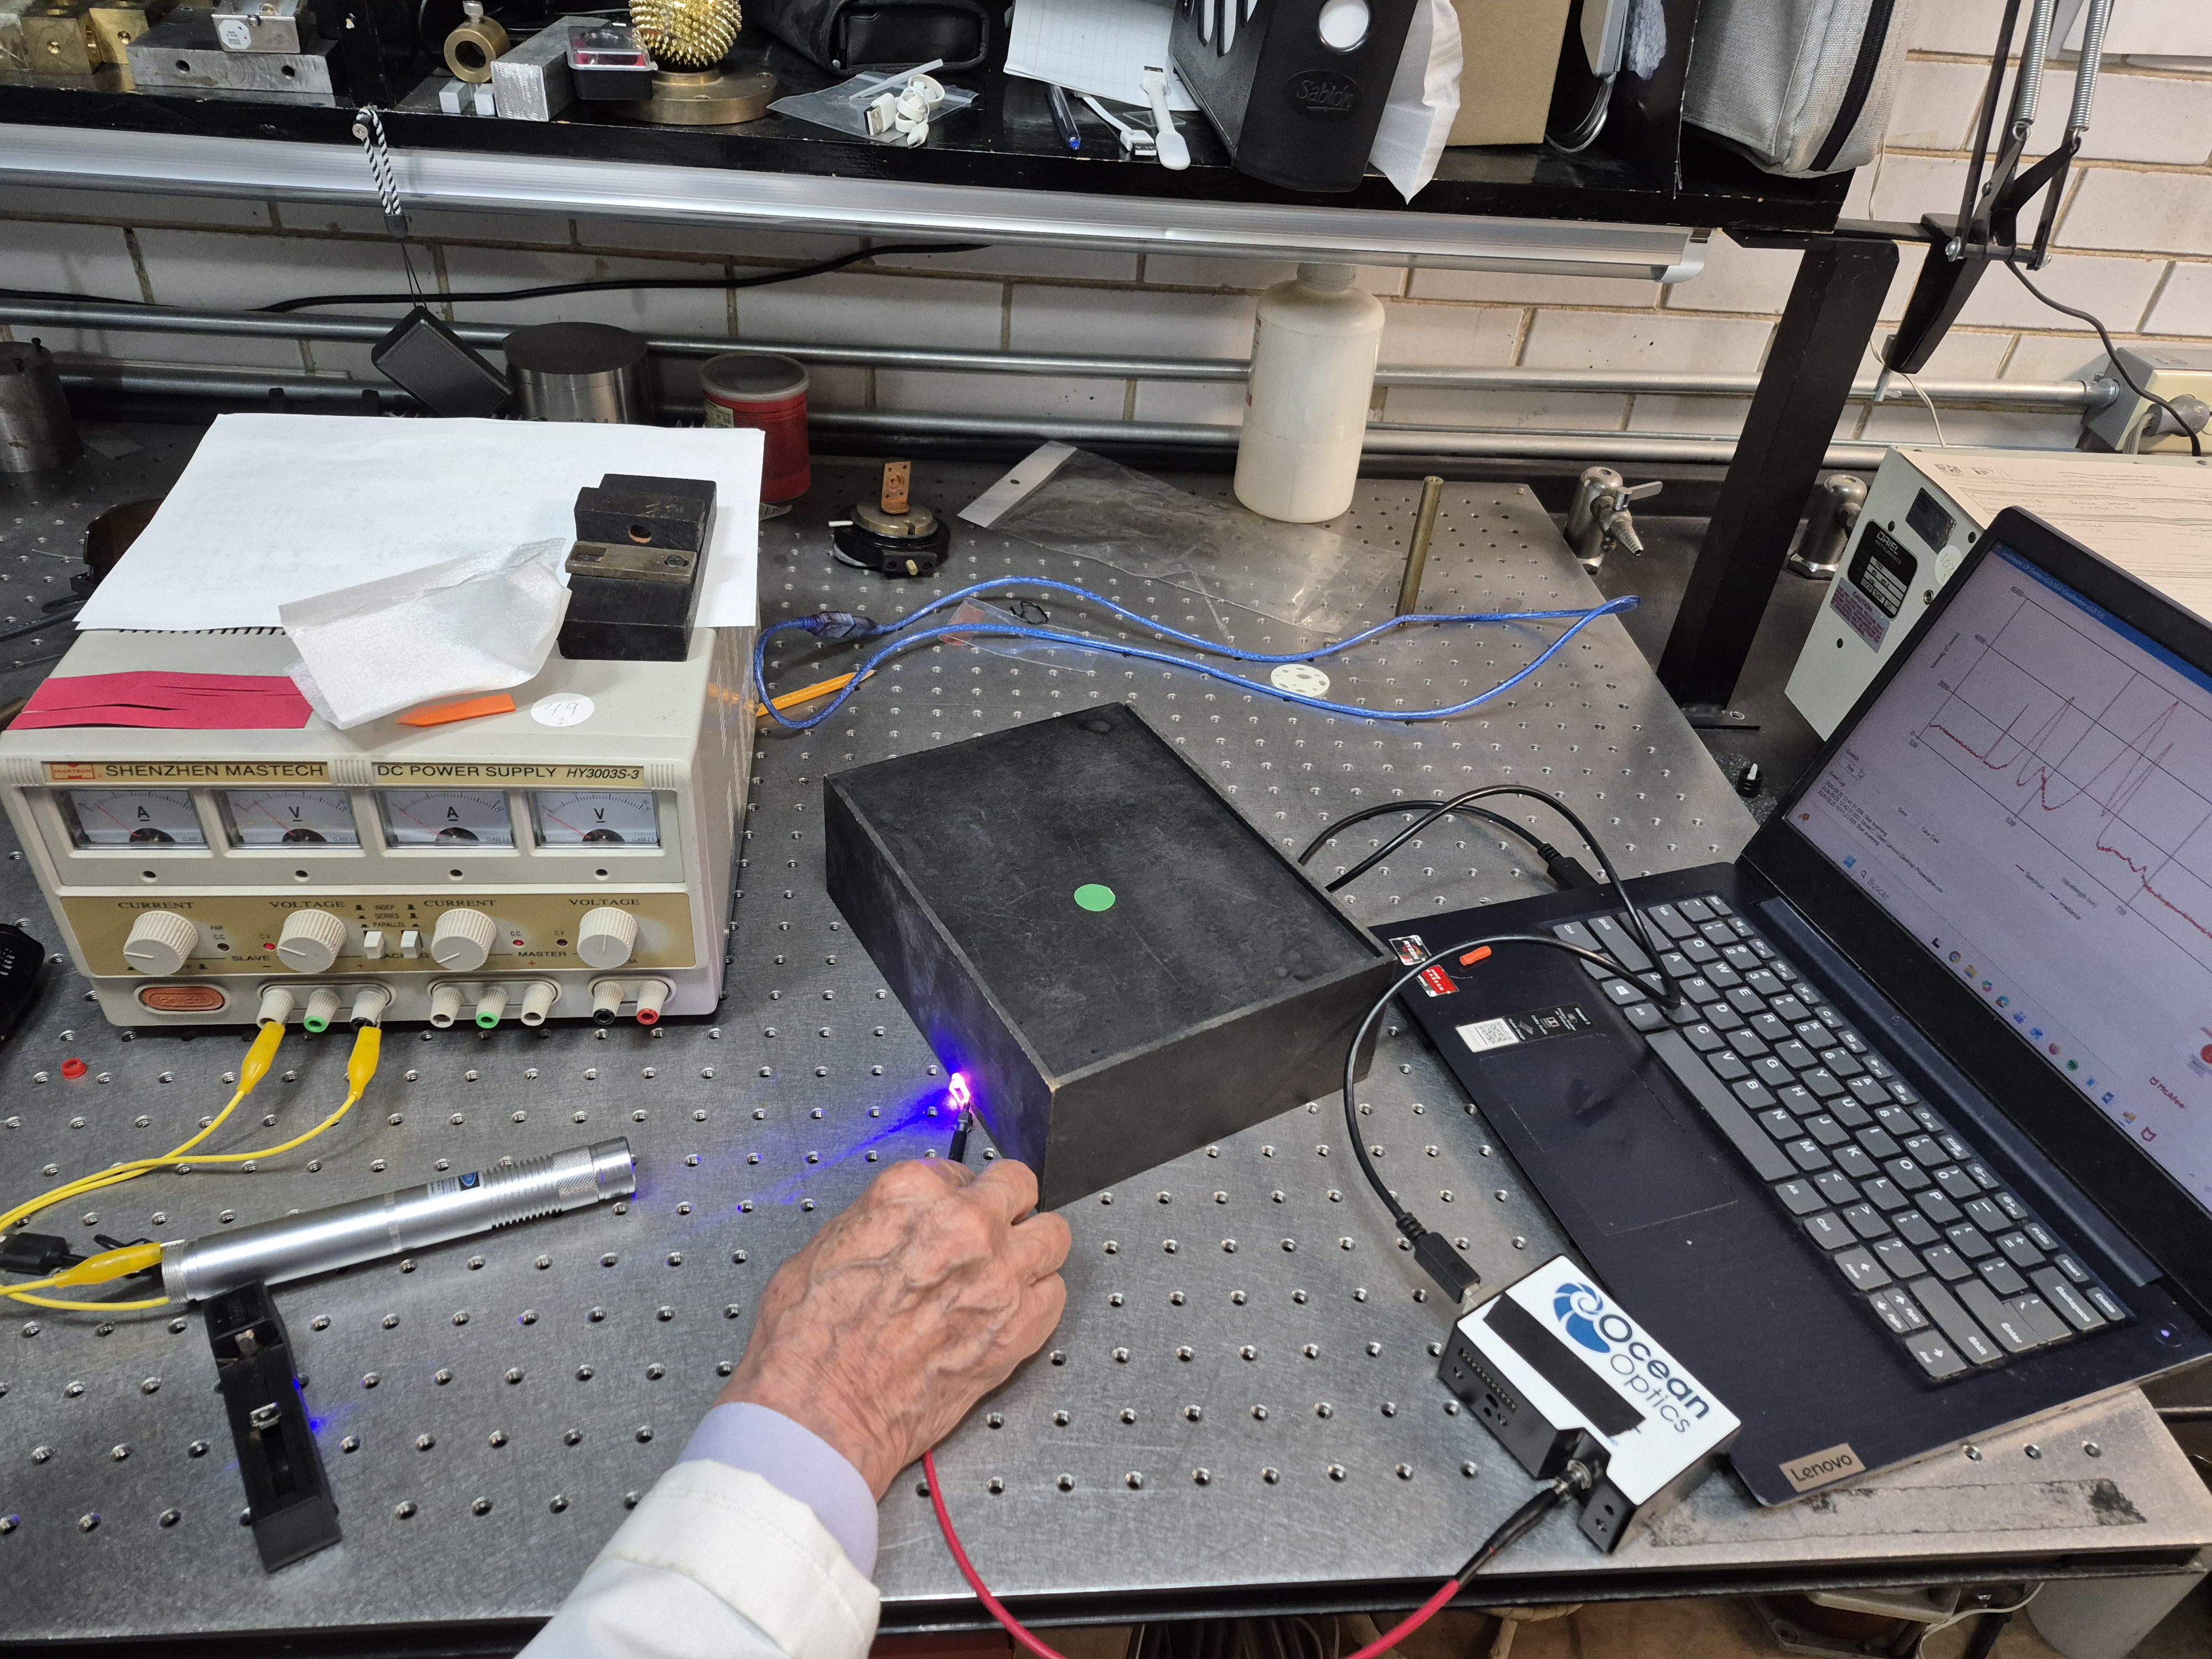
\includegraphics[scale=0.05]{figs/OceanOptics.jpg}
	\caption{Configuración manual de un láser y una fibra óptica para tomar espectros de emisión a través de un espectrómetro Ocean Optics.}
	\label{fig:OceanOptics}
\end{figure}

\noindent Se analizaron las siguientes siete muestras de tierras raras: un cristal mixto de fosfato y metafosfato de magnesio dopado con óxido de disprosio [Mg(PO$_3$)$_2$:Mg$_3$(PO$_4$)$_2$:Dy$_2$O$_3$ a una composición molar de $49.25\%$, $49.25\%$ y $1\%$, respectivamente], un cristal de niobato de litio dopado con óxido de disprosio [LiNbO$_3$:Dy$_2$O$_3$ a una composición molar de $99\%$ y $1.5\%$, respectivamente], un cristal de metafosfato de zinc dopado con óxido de disprosio [Zn(PO$_3$)$_2$:Dy$_2$O$_3$ a una composición molar de $99\%$ y $1\%$, respectivamente], un cristal mixto de fosfato y metafosfato de zinc dopado con óxido de samario [Zn(PO$_3$)$_2$:Zn$_3$(PO$_4$)$_2$:Sm$_2$O$_3$ a una composición molar de $49.5\%$, $49.5\%$ y $1\%$, respectivamente] un cristal de tetraborato de litio dopado con óxido de terbio [Li$_2$B$_4$O$_7$:Tb$_4$O$_7$, a una composición molar de $98\%$ y $2\%$, respectivamente], un cistal de metafosfato y ortofosfato de magnesio co-dopado con cloruro de estaño y óxido de europio [Mg(PO$_3$)$_2$:Mg$_3$(PO$_4$)$_2$:SnCl$_3$:Eu$_2$O$_3$, a una composición molar de $49\%$, $48\%$, $1\%$ y $3\%$, respectivamente] y un cistal de metafosfato y ortofosfato de zinc dopado con óxido de praseodimio [Zn(PO$_3$)$_2$:Zn$_3$(PO$_4$)$_2$:Pr$_2$O$_3$, a una composición molar de $49\%$, $49\%$ y $2\%$, respectivamente].

Primero se buscó en cada muestra la luz de excitación en la que se presentara el fenómeno de fotoluminiscencia; para ello, se utilizaron distintas lámparas de mano que emitían a una longitud de onda en específico, y se eligió la lámpara que mejor logró este efecto en el cristal. En el anexo (Figuras \ref{fig:Dy_Mg-fotos}-\ref{fig:Tb-fotos}) se muestran los cristales tanto a la intemperie como con el fenómeno de fotoluminiscencia, indicando el haz de excitación correspondiente.

Después se utilizó un espectrómetro de fluorescencia y luminiscencia Perkin Elmer LS55 (Figura \ref{fig:PerkinELmer}) para obtener el espectro de emisión de tres muestras: del disprocio en un fosfato y meta-fosfato de magnesio, el del samario y el del terbio. En la abertura del espectrómetro (Figura \ref{fig:abertura}) se colocó cada cristal y con un pedazo de papel (para ver la trayectoria del láser) se verificó que el haz incidiera sobre la mestra. Posteriormente se cerró este compartimiento y con el software FL Winlab (Figura \ref{fig:FL_Winlab}) se configuró el haz de excitación para cada muestra y se estableció que el recorrido del espectro fuera de los $420$ nm hasta los $850$ nm; se le dio en iniciar y se exportaron los datos del espectro de emisión (longitud de onda [nm] vs. intensidad).

Para el resto de las muestras se utilizó una configuración distinta ya que hubo problemas de comunicación entre el software FL Winlab y el espectrómetro. La nueva configuración se hizo manualmente (Figura \ref{fig:OceanOptics}); se usó una fuente de poder Shenzhen Mastech HY3003S-3 para potenciar el láser y un espectrómetro Ocean Optics con una fibra óptica para apuntar hacia el haz de emisión. Con el software OceanView se realizó la captura de los datos del espectro de emisión (longitud de onda [nm] vs. intensidad). Esta configuración se utilizó en las siguientes muestras: del disprosio en niobato de litio, del disprocio en metafosfato de zinc, el del samario (nuevamente, con el objetivo de realizar una comparación entre las dos configuraciones para obtener los espectros), el del europio y el del praseodimio.